\documentclass[sigconf,nonacm]{acmart}

\usepackage{booktabs}
\usepackage{makecell}
\usepackage{amsmath}
\usepackage{xcolor}

%% Placeholders for results still to be collected. Search for "TODO" / "\tbd".
\newcommand{\todo}[1]{\textcolor{red}{\textbf{[TODO:} #1\textbf{]}}}
\newcommand{\tbd}{\textcolor{red}{\textbf{TBD}}}

\settopmatter{printacmref=false}
\setcopyright{none}
\renewcommand\footnotetextcopyrightpermission[1]{}
\pagestyle{plain}
\setlength{\emergencystretch}{3em}

\begin{document}

\title{Training-Free Compression of Diffusion Transformers via Layer Looping}
\subtitle{CS 5787 Deep Learning: Interim Report}

\author{Jiacheng Yang}
\affiliation{%
  \institution{Cornell University}
  \city{New York}\state{NY}\country{USA}}
\email{jy2276@cornell.edu}

\author{Xinyi Lu}
\affiliation{%
  \institution{Cornell University}
  \city{New York}\state{NY}\country{USA}}
\email{xl2269@cornell.edu}

\author{Matthew Evan Lee}
\affiliation{%
  \institution{Cornell University}
  \city{New York}\state{NY}\country{USA}}
\email{mel328@cornell.edu}

\begin{abstract}
We study whether a frozen, pretrained image diffusion transformer can be compressed
without any training by deleting some of its transformer blocks and filling the
vacated depth slots with repeated applications of blocks that are kept. Following
Training-Free Looped Transformers~\cite{chen2026looped}, which re-applies mid-stack
layers of frozen language models as damped forward-Euler sub-steps, we apply the idea
to the class-conditional DiT-XL/2~\cite{peebles2023dit} at $256\times256$. We
implemented a reproducible, training-free pipeline. It profiles per-block feature change,
compares five block-replacement rules at a matched parameter budget, and measures
paired perceptual drift (LPIPS, TPIPS), distribution quality (FID, CLIP score) and
efficiency (unique parameters, FLOPs, latency). In a first 16-image validation run with
two of 28 blocks removed (7.1\% fewer unique parameters), simply skipping the blocks
stayed closest to the original samples (LPIPS $0.465$). Naive reuse of the preceding
block was significantly worse ($+0.128$ LPIPS, 95\% CI $[+0.054,+0.199]$). Damping the
reused update with $\alpha=0.5$ recovered about half of that gap. Training-free
exclusive self-attention~\cite{chng2026loopeddit} did not help.
\end{abstract}

\ccsdesc[500]{Computing methodologies~Computer vision}
\ccsdesc[300]{Computing methodologies~Neural networks}

\keywords{diffusion transformers, model compression, looped transformers, training-free inference}

\maketitle

%% ---------------------------------------------------------------------------
\section{Introduction}

\textbf{Problem.} Diffusion transformers (DiTs)~\cite{peebles2023dit,ma2024sit} reach
state-of-the-art image quality, but every one of their $N$ transformer blocks has its
own weights, which must be stored and kept in memory. We ask: \emph{can an off-the-shelf
DiT be made smaller without any retraining by deleting blocks and re-running blocks that
are kept in their place?} If recurrence can stand in for distinct blocks, the model's
storage and parameter memory shrink while its computational depth is preserved.

\textbf{Basis.} Our primary reference is \emph{Training-Free Looped
Transformers}~\cite{chen2026looped}. Chen et al.\ observe that a pre-norm residual
block $L(x)=x+F_L(x)$ is exactly one forward-Euler step of size $h=1$ on the ODE
$\dot x=F_L(x)$. Naively re-applying a block integrates that ODE to $t=K$, outside the
regime later layers were trained on, and degrades accuracy. Replacing one step by $K$
damped sub-steps of size $1/K$ (or a Runge--Kutta blend of the two) instead lets a frozen
LLM loop a contiguous window of about four mid-depth layers. Their goal is to spend
\emph{more} compute on a fixed checkpoint. Ours is the reverse: we \emph{remove}
blocks and use looping to recover the lost depth. The backbone is
DiT-XL/2~\cite{peebles2023dit}, a 28-block, 675M-parameter class-conditional latent
diffusion transformer. TeaCache~\cite{liu2025teacache} motivates our block-selection
signal: it shows that relative $L_1$ changes of DiT features vary strongly across
timesteps and can identify redundant computation without training. ELT~\cite{goyal2026elt}
and Looped-DiT~\cite{chng2026loopeddit} show that \emph{trained} weight-shared looped
DiTs can match much larger models. Both need training (intra-loop self-distillation, or
deep supervision with self-modulating attention). We test whether their key ingredient,
exclusive self-attention (XSA), helps when it is added without training. We measure
aspect-specific perceptual drift with TPIPS~\cite{wang2026tpips}.

%% ---------------------------------------------------------------------------
\section{Problem Formulation}

\textbf{Generator.} Let $f_\theta$ be the pretrained DiT-XL/2 noise predictor with
blocks $B_0,\dots,B_{N-1}$ ($N=28$, hidden width $d=1152$, $T=256$ tokens per
$32\times32\times4$ VAE latent). Given a class label $y$, an initial latent
$z\sim\mathcal N(0,I)$ and sampler noise $\xi$, the fixed sampler $\mathcal S$ (50-step
ancestral DDPM sampling~\cite{ho2020ddpm} with classifier-free guidance~\cite{ho2021cfg},
scale $s=4$) followed by the VAE decoder yields an image
$x=G(f_\theta;y,z,\xi)\in[-1,1]^{3\times256\times256}$. Fixing $(y,z,\xi)$ per sample
makes $G$ deterministic, so two generators can be compared image by image.

\textbf{Objective.} Find a compressed generator $\tilde f$ built only from the frozen
weights $\theta$ (no gradient updates), with unique parameter count
$P(\tilde f)\le(1-\rho)P(f_\theta)$ for budget $\rho$, minimizing the expected distance
\begin{equation}
  \mathcal D(\tilde f)=\mathbb E_{y,z,\xi}\,
  d\big(G(\tilde f;y,z,\xi),\,G(f_\theta;y,z,\xi)\big)
\end{equation}
while keeping the sample distribution close to real data. We report compute (FLOPs,
latency) alongside, since looping keeps compute while removal reduces it.

\textbf{Data.} The method needs no training data. Conditioning inputs are ImageNet-1k
class labels with fixed seeds, defined once in a shared protocol file. The pilot uses
eight classes (golden retriever, otter, red panda, geyser, macaw, valley, balloon,
arctic fox) and three disjoint seed sets: \emph{calibration} (16 images) to select
blocks and score candidates, \emph{validation} (16) to choose settings, and a held-out
\emph{test} split (64) evaluated once with frozen choices. A separate \emph{fid} split
has one image per class for all 1000 classes; the final study uses 500 of these
(every second class). Real-image references are the ImageNet validation set (50
images per generated class, bicubic-resized and center-cropped to 256) and the ADM
ImageNet-256 statistics~\cite{dhariwal2021adm}. All runs fix FP32, deterministic
kernels, the DiT commit, the checkpoint hash and the VAE revision. Every run checks
that the protocol, code and software environment are unchanged.

\textbf{Metrics.}
(i)~\emph{Paired LPIPS}~\cite{zhang2018lpips} (AlexNet, v0.1) between $\tilde x$ and
$x$ for the same $(y,z,\xi)$, our main validation criterion: lower means closer to the
original, not better quality.
(ii)~\emph{TPIPS}~\cite{wang2026tpips}: paired, text-conditioned distances for the
aspects \emph{overall}, \emph{shape} and \emph{texture}.
(iii)~\emph{FID}~\cite{heusel2017fid}: Clean-FID~\cite{parmar2022cleanfid} against the
real ImageNet references, FID-500 against the original model's own samples, and FID
against the ADM statistics. With $n<2048$ the covariance is rank deficient, so FID is
used only to compare methods with each other.
(iv)~\emph{CLIP score}~\cite{radford2021clip,hessel2021clipscore}:
$100\cdot\mathbb E[\max(\cos(E_I(x),E_T(\text{``a photo of a }\{y\}\text{''})),0)]$
with ViT-B/32, measuring class fidelity.
(v)~\emph{Efficiency}: unique parameters, serialized checkpoint size, DiT FLOPs per
sampling run (a multiply-add counts as two operations; VAE and elementwise operations are
excluded), synchronized end-to-end latency and peak memory.

%% ---------------------------------------------------------------------------
\section{Method}

\textbf{DiT block.} Each block is an adaLN-Zero transformer
block~\cite{peebles2023dit}. With conditioning $c=e_t(t)+e_y(y)$ and
$(\beta_1,\gamma_1,a_1,\beta_2,\gamma_2,a_2)=W_\ell c$,
\begin{align}
  h' &= h + a_1\odot \mathrm{Attn}_\ell\big((1+\gamma_1)\odot\mathrm{LN}(h)+\beta_1\big),\\
  B_\ell(h,c) &= h' + a_2\odot \mathrm{MLP}_\ell\big((1+\gamma_2)\odot\mathrm{LN}(h')+\beta_2\big).
\end{align}
As in~\cite{chen2026looped}, $B_\ell(h,c)=h+F_\ell(h,c)$ is one Euler step of size 1 on
$\dot h=F_\ell(h,c)$.

\textbf{Block selection.} We run the original model on the calibration split and
record, for every sample, block $\ell$ and timestep $t$, the normalized feature change
\begin{equation}
  r_\ell(t)=\frac{\lVert h_{\ell+1}(t)-h_\ell(t)\rVert_1}{\lVert h_\ell(t)\rVert_1+\epsilon},
\end{equation}
analogous to TeaCache's relative $L_1$ indicator~\cite{liu2025teacache}. We average it
separately over the conditional and unconditional CFG branches, then over samples within
each timestep, then over timesteps with equal weight. The $k$ blocks with the smallest
score form the removed set $R$; blocks $0$ and $N-1$ are never removed. Unique
parameters fall by $|R|$ blocks ($23.9$M each).

\textbf{Slot replacement rules (single blocks).} Let
$\pi(\ell)=\max\{j<\ell: j\notin R\}$ be the nearest preceding kept block. The forward
pass keeps $h_{\ell+1}=B_\ell(h_\ell,c)$ for $\ell\notin R$ and, for $\ell\in R$, uses:
\begin{align}
\text{Removal:}\quad & h_{\ell+1}=h_\ell,\\
\text{Loop:}\quad & h_{\ell+1}=B_{\pi(\ell)}(h_\ell,c),\\
\text{Damped:}\quad & h_{\ell+1}=h_\ell+\alpha\big(B_{\pi(\ell)}(h_\ell,c)-h_\ell\big),
\end{align}
where damped is an Euler step of size $\alpha\in[0,1]$ with the borrowed field
$F_{\pi(\ell)}$ ($\alpha=0$ gives removal and $\alpha=1$ gives loop). Weights of
$\pi(\ell)$ are stored once and shared across its depth slots.

\textbf{XSA reuse.} Exclusive self-attention~\cite{chng2026loopeddit} removes each
token's own value direction from its attention output. For head $h$ with values
$v_{j,h}$ and weights $a_{ij,h}$, and $\hat v_{i,h}=v_{i,h}/\lVert v_{i,h}\rVert_2$,
\begin{equation}
  z_{i,h}=\big(I-\hat v_{i,h}\hat v_{i,h}^{\top}\big)\textstyle\sum_j a_{ij,h}v_{j,h}.
\end{equation}
Looped-DiT trains this inside its looped blocks. We apply it training-free and only at
replacement slots: $h_{\ell+1}=B^{\mathrm{XSA}}_{\pi(\ell)}(h_\ell,c)$. The projection
is inserted before the output projection, and the original block call is left
unchanged elsewhere.

\textbf{Window looping.} Closer to Chen et al.'s construction, a second family replaces
a contiguous window $[a,b]$. It keeps a central subset $K_w\subset[a,b]$, discards
$D=[a,b]\setminus K_w$ (budget $|D|\in\{2,4,6\}$) and iterates
$g=B_{k_m}\circ\dots\circ B_{k_1}$ over the kept blocks $K$ times (block mode), or each
kept block $K$ times in turn (layer mode). The three strategies are:
\begin{align}
\text{naive:}\quad & x\leftarrow g(x)\quad (K\text{ times}),\\
\text{damped:}\quad & x\leftarrow x+h\,(g(x)-x)\quad (K\text{ times},\ h=1/K),\\
\text{anchored:}\quad & x\leftarrow \beta\, g(x_0)+(1-\beta)\,\Phi_h^{K}(x_0),
\end{align}
where $\Phi_h(x)=x+h(g(x)-x)$. The anchored strategy is the $K$-stage Runge--Kutta
interpolation of~\cite[Eq.~16]{chen2026looped}, computed with $K$ evaluations of $g$.
We screen candidate windows on the calibration split before generating any images.
The original sampler is run once to cache the states $(x_t,t,y)$ it visits. Each
candidate is then scored by its one-step noise-prediction error on those states,
$\mathrm{err}=\lVert\hat\epsilon_{\text{cand}}-\hat\epsilon_{\text{ref}}\rVert^2/
\lVert\hat\epsilon_{\text{ref}}\rVert^2$, averaged over timestep buckets. The best
candidates per budget, together with equal-parameter removal controls, go to
validation. There a configuration is frozen only if its paired LPIPS improvement over
removal has a bootstrap 95\% interval below zero.

%% ---------------------------------------------------------------------------
\section{Preliminary Results}

\textbf{Setup.} One validation run on an NVIDIA T4 (Colab): calibration profiling on
the 16 calibration images, then all five rules with the same removed set and the 16
validation images. Removing $k=2$ blocks means $\rho=7.1\%$; damped uses the fixed pilot
value $\alpha=0.5$. LPIPS and PSNR are computed from the run's lossless 8-bit PNG
previews of the same images. \todo{replace with pipeline LPIPS on the saved FP32
tensors (\texttt{team\_\allowbreak{}pipeline.\allowbreak{}cli evaluate}) and update Table~\ref{tab:prelim} and the
paired intervals.} FLOPs and parameter counts are computed exactly from the
architecture.

\begin{figure}[t]
  \centering
  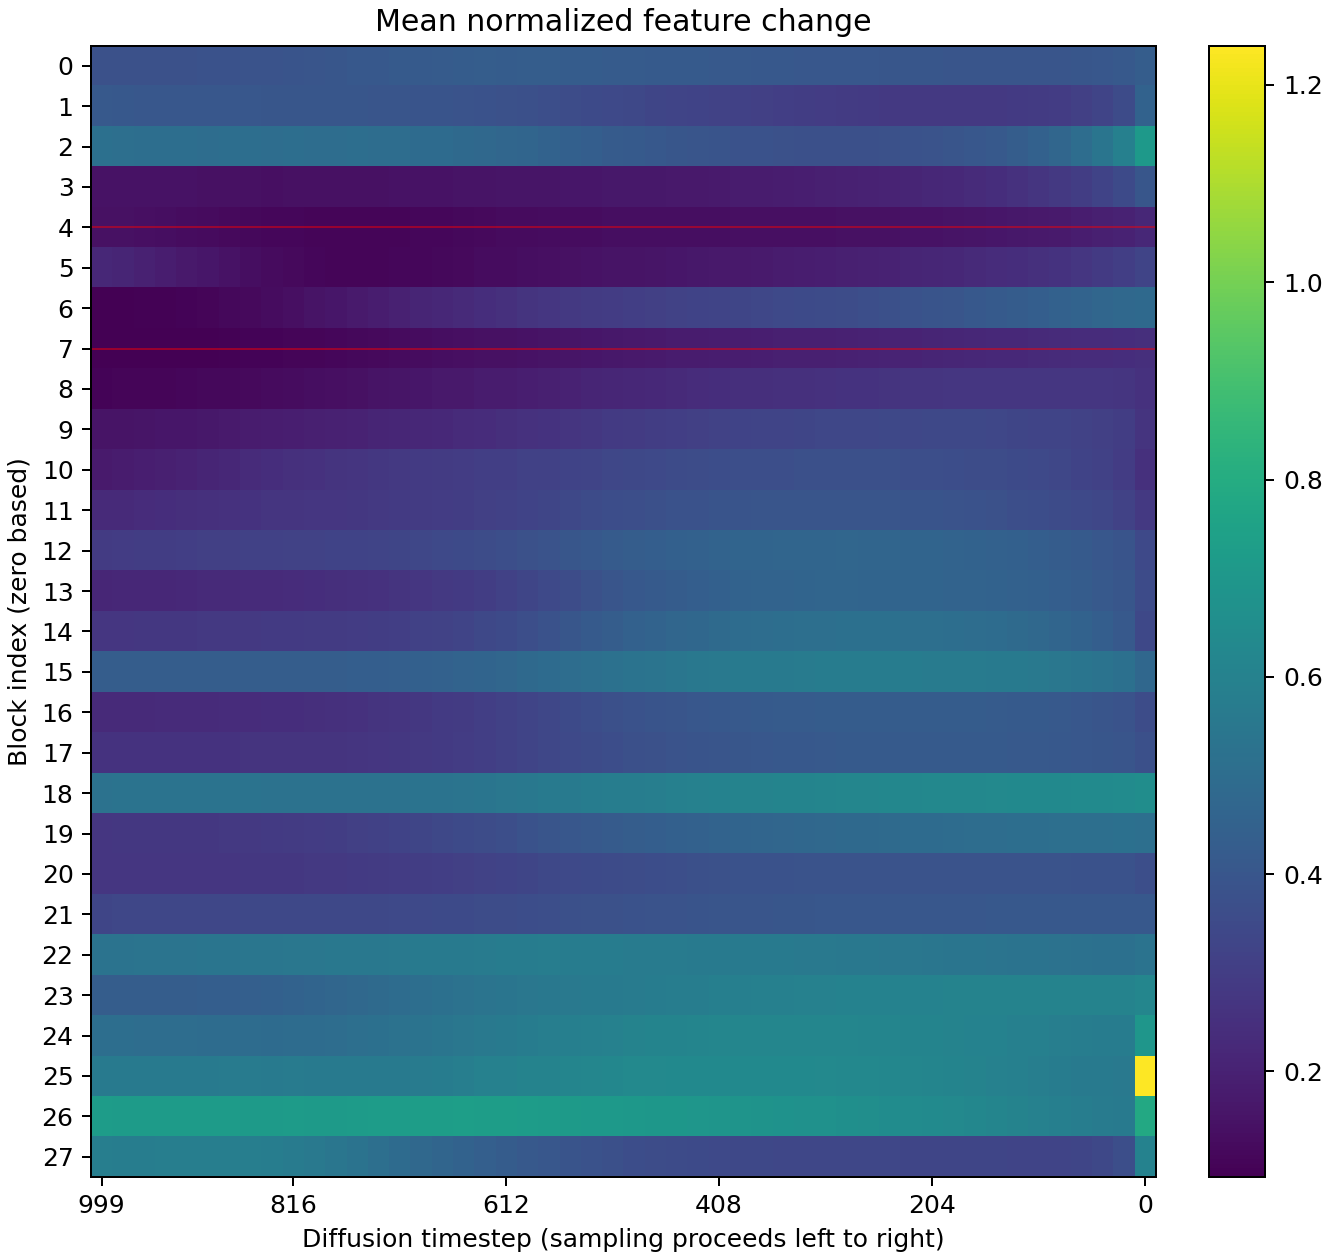
\includegraphics[width=\linewidth]{figures/heatmap.png}
  \caption{Mean normalized feature change $r_\ell(t)$ of DiT-XL/2 on the calibration
  split (rows: blocks; columns: timesteps in sampling order). Red lines mark the two
  selected blocks, 4 and 7.}
  \Description{Heatmap with blocks on the vertical axis and diffusion timesteps on the
  horizontal axis; early blocks 3 to 8 show the smallest changes.}
  \label{fig:heatmap}
\end{figure}

\textbf{Where are the redundant blocks?} Figure~\ref{fig:heatmap} shows that the
smallest per-block updates are in \emph{early} blocks 3--8, especially at high-noise
timesteps. The largest updates are in blocks 2, 18 and 22--27. The selected blocks
(4 and 7) sit at depth fractions $0.14$--$0.25$. This differs from the mid-depth band
($0.45$--$0.60$) that Chen et al.\ find best for looping LLMs~\cite{chen2026looped}, so
their depth rule should not be assumed to carry over to DiTs. Our window screening
therefore covers windows starting from block 4 onward.

\begin{table}[t]
  \caption{Validation pilot, 2 blocks (4, 7) replaced, 16 paired images. LPIPS/PSNR are
  measured against the original model's image for the same label and seeds (mean $\pm$
  std). GFLOPs are per CFG forward pass (batch 2, multiply-add $=2$). Latency is T4,
  50 steps plus VAE decode.}
  \label{tab:prelim}
  \small
  \setlength{\tabcolsep}{2.2pt}
  \begin{tabular}{lrrrrrr}
    \toprule
    Method & Params & Evals & GFLOPs & Latency (s) & LPIPS$\downarrow$ & PSNR$\uparrow$\\
    \midrule
    Original & 675.1M & 28 & 474.5 & $8.60\pm0.19$ & -- & --\\
    Removal  & 627.3M & 26 & 440.6 & $8.11\pm0.31$ & $\mathbf{0.465}\pm0.134$ & \textbf{13.9}\\
    Loop     & 627.3M & 28 & 474.5 & $8.69\pm0.30$ & $0.593\pm0.126$ & 11.6\\
    Damped   & 627.3M & 28 & 474.5 & $8.68\pm0.27$ & $0.530\pm0.132$ & 12.8\\
    XSA reuse& 627.3M & 28 & 474.5 & $8.71\pm0.30$ & $0.598\pm0.123$ & 11.4\\
    \bottomrule
  \end{tabular}
\end{table}

\textbf{Efficiency.} All compressed models store 26 unique blocks (47.8M fewer parameters,
$-7.1\%$). Our FLOP count for the original, $474.5$ GFLOPs per CFG forward, equals
$2\times2\times118.6$: the 118.6 GFLOPs DiT reports~\cite{peebles2023dit}, doubled for the
two CFG branches and doubled again because we count a multiply-add as two operations.
This serves as a check on the estimator. Removal also cuts FLOPs ($-7.1\%$) and latency
($-5.6\%$). The looped rules keep the original FLOPs and run about 1\% slower than the
original, because of the wrapper overhead.

\textbf{Fidelity.} Removal stays closest to the original (Table~\ref{tab:prelim}).
Per-image paired differences, with bootstrap 95\% intervals over the 16 images, are:
loop $-$ removal $=+0.128$ $[+0.054,+0.199]$ (loop worse on 12/16 images); damped $-$
removal $=+0.065$ $[+0.016,+0.121]$; loop $-$ damped $=+0.063$ $[+0.017,+0.106]$;
XSA $-$ loop $=+0.005$ $[-0.033,+0.045]$. So damping by $\alpha=0.5$ removes about half
of the damage from naive reuse. This matches Chen et al.'s finding that undamped
re-application leaves the trained regime~\cite{chen2026looped}: borrowing a whole extra
Euler step of size 1 from a neighbouring block overshoots, and a half step overshoots
less. Training-free XSA is indistinguishable from plain looping. In Looped-DiT its
benefit relies on training the looped blocks~\cite{chng2026loopeddit}.

\begin{figure}[t]
  \centering
  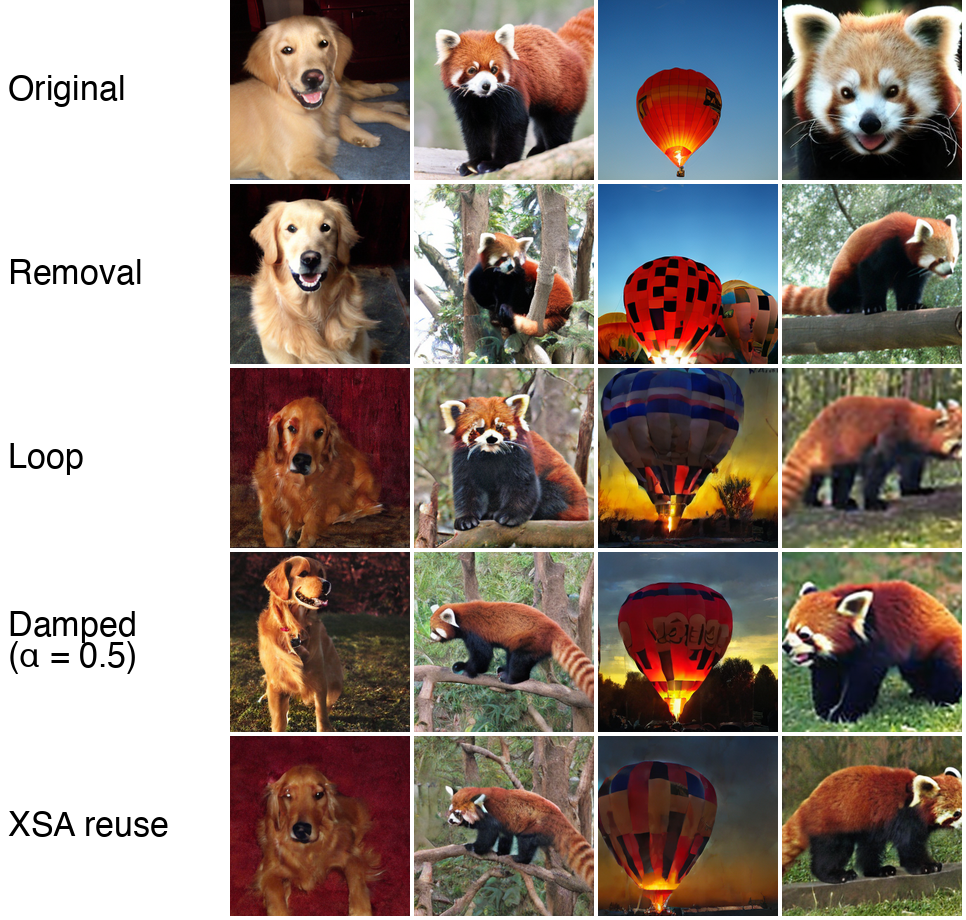
\includegraphics[width=\linewidth]{figures/qualitative.png}
  \caption{Paired validation samples (columns share class, initial noise and sampler
  noise). Removing two early blocks changes global layout. Loop and XSA reuse also add
  over-sharpened textures and colour shifts; damped looping is in between.}
  \Description{Grid of generated images: five rows (original, removal, loop, damped, XSA
  reuse) by four columns (golden retriever, red panda, hot-air balloon, red panda).}
  \label{fig:qual}
\end{figure}

\textbf{Qualitative.} Even removal has high absolute LPIPS ($\approx0.46$),
because removing early blocks changes the noise prediction at high-noise steps. The
ancestral sampler amplifies that change into different composition and pose
(Figure~\ref{fig:qual}). Class identity is mostly preserved. The looped rules add
high-frequency artifacts and saturation shifts, and occasionally lose the object (otter,
valley). Low feature change therefore does not imply that a block can be safely reused
(or removed): the blocks that change features least still move samples substantially.

\textbf{Perceptual aspects and random control.}
Table~\ref{tab:aspects} adds TPIPS~\cite{wang2026tpips} and a control that removes two
randomly chosen blocks (same budget) with ordinary looping.
\todo{run \texttt{team\_\allowbreak{}pipeline.\allowbreak{}cli extended -{}-tpips-factors overall shape texture} on
the validation split; add the random-selection control; fill Table~\ref{tab:aspects} and
state whether feature-change selection beats random selection.}

\begin{table}[t]
  \caption{TPIPS against the original images (lower is closer) and a random-selection
  control, validation split, 2 blocks replaced. \tbd{} = to be filled.}
  \label{tab:aspects}
  \small
  \begin{tabular}{lccc}
    \toprule
    Method & TPIPS overall & TPIPS shape & TPIPS texture\\
    \midrule
    Removal          & \tbd & \tbd & \tbd\\
    Loop             & \tbd & \tbd & \tbd\\
    Damped           & \tbd & \tbd & \tbd\\
    XSA reuse        & \tbd & \tbd & \tbd\\
    Random + loop    & \tbd & \tbd & \tbd\\
    \bottomrule
  \end{tabular}
\end{table}

\textbf{Damping strength and block position.} \todo{sweep
$\alpha\in\{0.25,0.5,0.75\}$ for the damped rule and compare the early blocks chosen
by calibration with mid-depth blocks (Figure~\ref{fig:heatmap}); report validation
LPIPS per setting.}

\textbf{Window looping.} Table~\ref{tab:window} reports the best screened window per
budget against equal-parameter removal.
\todo{run \texttt{loop\_\allowbreak{}compression.\allowbreak{}sensitivity blocks/\allowbreak{}windows} and
\texttt{loop\_\allowbreak{}compression.\allowbreak{}drive validate/\allowbreak{}freeze}; fill Table~\ref{tab:window} with the
frozen configuration per budget, its screening error and the paired LPIPS difference
versus removal with its bootstrap interval.}

\begin{table}[t]
  \caption{Window looping on validation: frozen configuration per budget versus the
  strongest equal-parameter removal. $\Delta$ = loop $-$ removal paired LPIPS
  (95\% CI). \tbd{} = to be filled.}
  \label{tab:window}
  \small
  \setlength{\tabcolsep}{3pt}
  \begin{tabular}{cllcc}
    \toprule
    $|D|$ & Window / kept & Strategy ($K$, $h$, $\beta$) & LPIPS & $\Delta$ (95\% CI)\\
    \midrule
    2 & \tbd & \tbd & \tbd & \tbd\\
    4 & \tbd & \tbd & \tbd & \tbd\\
    6 & \tbd & \tbd & \tbd & \tbd\\
    \bottomrule
  \end{tabular}
\end{table}

\textbf{Held-out test and distribution quality.} Table~\ref{tab:final} reports the
frozen configurations on the 64-image test split and on 500 images of the \emph{fid}
split. \todo{run \texttt{loop\_\allowbreak{}compression.\allowbreak{}final test/\allowbreak{}timing/\allowbreak{}fid/\allowbreak{}report} (and the
five-rule comparison with \texttt{-{}-split test}); fill Table~\ref{tab:final}; add
Clean-FID against real ImageNet images via \texttt{team\_\allowbreak{}pipeline.\allowbreak{}cli fid-reference}
and \texttt{extended}.}

\begin{table}[t]
  \caption{Frozen configurations on held-out data. Test LPIPS on 64 paired images;
  FID-500 and CLIP score on the \emph{fid} split; latency from interleaved repeated
  timing. \tbd{} = to be filled.}
  \label{tab:final}
  \small
  \setlength{\tabcolsep}{2.5pt}
  \begin{tabular}{lccccc}
    \toprule
    Method & \makecell{Test\\LPIPS$\downarrow$} & \makecell{FID vs\\orig.$\downarrow$} &
      \makecell{FID vs\\ADM$\downarrow$} & CLIP$\uparrow$ & \makecell{Latency\\(s)}\\
    \midrule
    Original          & --   & 0    & \tbd & \tbd & \tbd\\
    Removal           & \tbd & \tbd & \tbd & \tbd & \tbd\\
    Damped            & \tbd & \tbd & \tbd & \tbd & \tbd\\
    Best window loop  & \tbd & \tbd & \tbd & \tbd & \tbd\\
    \bottomrule
  \end{tabular}
\end{table}

\textbf{Summary.} \todo{once Tables~\ref{tab:aspects}--\ref{tab:final} are filled,
summarize whether any training-free looping rule beats equal-parameter removal at each
budget, and at what compute cost.}

\bibliographystyle{ACM-Reference-Format}
\begin{thebibliography}{99}

\bibitem{chen2026looped}
Lizhang Chen, Jonathan Li, Chen Liang, Ni Lao, and Qiang Liu. 2026.
Training-Free Looped Transformers. arXiv:2605.23872.

\bibitem{peebles2023dit}
William Peebles and Saining Xie. 2023.
Scalable Diffusion Models with Transformers. In \emph{ICCV}. 4195--4205.

\bibitem{ma2024sit}
Nanye Ma, Mark Goldstein, Michael S. Albergo, Nicholas M. Boffi, Eric Vanden-Eijnden,
and Saining Xie. 2024. SiT: Exploring Flow and Diffusion-based Generative Models with
Scalable Interpolant Transformers. In \emph{ECCV}.

\bibitem{liu2025teacache}
Feng Liu, Shiwei Zhang, Xiaofeng Wang, Yujie Wei, Haonan Qiu, Yuzhong Zhao, Yingya Zhang,
Qixiang Ye, and Fang Wan. 2025. Timestep Embedding Tells: It's Time to Cache for Video
Diffusion Model. In \emph{CVPR}.

\bibitem{goyal2026elt}
Sahil Goyal, Swayam Agrawal, Gautham Govind Anil, Prateek Jain, Sujoy Paul, and Aditya
Kusupati. 2026. ELT: Elastic Looped Transformers for Visual Generation.
arXiv:2604.09168.

\bibitem{chng2026loopeddit}
Yong Xien Chng, Tianyi Chen, Wenwen Tong, Haiwen Diao, Zhongang Cai, Lei Yang, Ziwei Liu,
Lewei Lu, Dahua Lin, and Gao Huang. 2026. Looped Diffusion Transformer.
arXiv:2609.40305.

\bibitem{wang2026tpips}
Sheng-Yu Wang, Yotam Nitzan, Aaron Hertzmann, Jun-Yan Zhu, Eli Shechtman, Alexei A. Efros,
and Richard Zhang. 2026. The Many Senses of Visual Similarity: A Text-Prompted Image
Perceptual Metric. arXiv:2607.18237.

\bibitem{ho2020ddpm}
Jonathan Ho, Ajay Jain, and Pieter Abbeel. 2020. Denoising Diffusion Probabilistic
Models. In \emph{NeurIPS}.

\bibitem{ho2021cfg}
Jonathan Ho and Tim Salimans. 2021. Classifier-Free Diffusion Guidance. In
\emph{NeurIPS Workshop on Deep Generative Models}.

\bibitem{dhariwal2021adm}
Prafulla Dhariwal and Alex Nichol. 2021. Diffusion Models Beat GANs on Image Synthesis.
In \emph{NeurIPS}.

\bibitem{zhang2018lpips}
Richard Zhang, Phillip Isola, Alexei A. Efros, Eli Shechtman, and Oliver Wang. 2018.
The Unreasonable Effectiveness of Deep Features as a Perceptual Metric. In \emph{CVPR}.

\bibitem{heusel2017fid}
Martin Heusel, Hubert Ramsauer, Thomas Unterthiner, Bernhard Nessler, and Sepp
Hochreiter. 2017. GANs Trained by a Two Time-Scale Update Rule Converge to a Local Nash
Equilibrium. In \emph{NeurIPS}.

\bibitem{parmar2022cleanfid}
Gaurav Parmar, Richard Zhang, and Jun-Yan Zhu. 2022. On Aliased Resizing and Surprising
Subtleties in GAN Evaluation. In \emph{CVPR}.

\bibitem{radford2021clip}
Alec Radford, Jong Wook Kim, Chris Hallacy, Aditya Ramesh, Gabriel Goh, Sandhini Agarwal,
Girish Sastry, Amanda Askell, Pamela Mishkin, Jack Clark, Gretchen Krueger, and Ilya
Sutskever. 2021. Learning Transferable Visual Models From Natural Language Supervision.
In \emph{ICML}.

\bibitem{hessel2021clipscore}
Jack Hessel, Ari Holtzman, Maxwell Forbes, Ronan Le Bras, and Yejin Choi. 2021.
CLIPScore: A Reference-free Evaluation Metric for Image Captioning. In \emph{EMNLP}.

\end{thebibliography}

\end{document}
